\section{Motivation and Scope}

There has been a strong desire for a more space- and/or runtime-efficient
representation for \code{map} among C++ users for some time now.  This has
motivated discussions among the members of SG14 resulting in a
paper\footnote{See P0038R0,
  \href{http://www.open-std.org/jtc1/sc22/wg21/docs/papers/2015/p0038r0.html}{here}.},
numerous articles and talks, and an implementation in Boost,
\code{boost::container::flat_map}\footnote{Part of Boost.Container,
  \href{http://www.boost.org/doc/libs/1_61_0/doc/html/container.html}{here}.}.
Virtually everyone who makes games, embedded, or system software in C++ uses
the Boost implementation or one that they rolled themselves.\\

Here are some numbers that show why.  The graphs that follow show runtimes for
different \code{map}-like associative containers.  The containers used are
Boost.FlatMap, \code{map}, and two thin wrappers over a sorted \code{vector};
the ``custom pair'' version of the sorted \code{vector} uses a simple
\code{struct} instead of \code{pair} for its value type.  All containers use
an \code{int} as the key type and an \code{int} or a \code{struct} with 5
\code{double}s for the value type.\\

All the graphs below were produced on Windows with MSVC 2015.  Similar results
were obtained on Linux, with Clang 3.9 and libc++, and with g++ 4.8.4 and
libstdc++.\\

These first four graphs cover the \code{int}-value-type case.  The first graph
shows insertion of N elements with random keys; the second shows full
iteration across all N elements; the third shows \code{map.find()} called once
for each key used in the original insertions; and the fourth shows erasure of
all N elements, by the keys used in the original insertions.

\begin{center}
    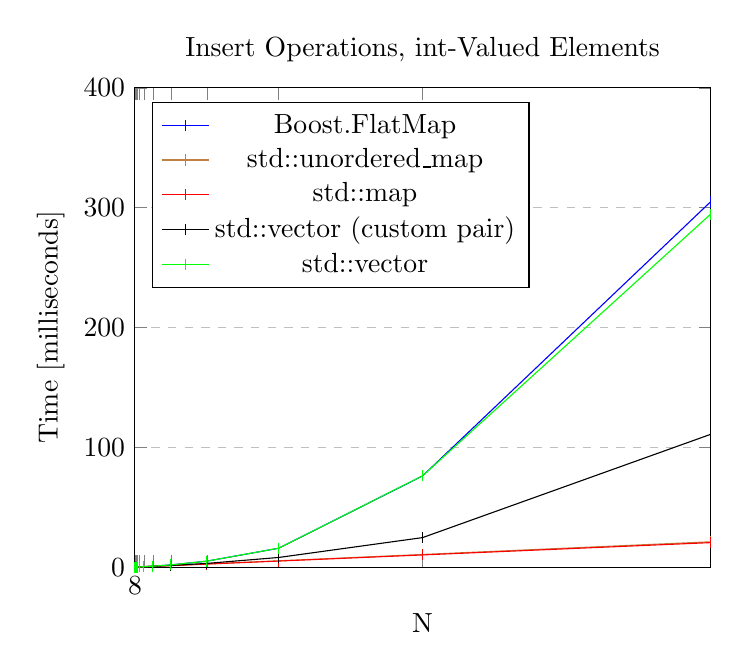
\begin{tikzpicture}
    \begin{axis}[
        width=3.5in,
        title={Insert Operations, int-Valued Elements},
        xlabel={N},
        ylabel={Time [milliseconds]},
        xmin=0, xmax=32768,
        ymin=0, ymax=400.0,
        xtick={8,16,32,64,128,256,512,1024,2048,4096,8192,16384,32768,65536},
        xticklabels={8,,,,,,,,,,,,,},
        ytick={0.0,100.0,200.0,300.0,400.0,500.0},
        legend pos=north west,
        ymajorgrids=true,
        grid style=dashed,
        scaled x ticks=false,
        scaled y ticks=true,
        legend entries={Boost.FlatMap,std::unordered\_map,std::map,std::vector (custom pair),std::vector},
        ]

    \addplot[color=blue,mark=|,]
        coordinates {(8,0.0059224)(16,0.010336)(32,0.0211488)(64,0.0436082)(128,0.0773848)(256,0.169297)(512,0.335145)(1024,0.76154)(2048,1.83041)(4096,4.93908)(8192,15.7292)(16384,76.0957)(32768,304.713)};

    \addplot[color=brown,mark=|,]
        coordinates {(8,0.007111)(16,0.0138582)(32,0.0248076)(64,0.0412908)(128,0.0816028)(256,0.161965)(512,0.360402)(1024,0.691291)(2048,1.34357)(4096,2.63649)(8192,5.25462)(16384,10.5295)(32768,21.1176)};

    \addplot[color=red,mark=|,]
        coordinates {(8,0.005406)(16,0.0103222)(32,0.0206594)(64,0.0421836)(128,0.0758348)(256,0.155035)(512,0.308779)(1024,0.618069)(2048,1.24506)(4096,2.51085)(8192,5.02993)(16384,10.1434)(32768,20.4145)};

    \addplot[color=black,mark=|,]
        coordinates {(8,0.0052384)(16,0.0104622)(32,0.0200862)(64,0.0370994)(128,0.0751898)(256,0.151988)(512,0.307287)(1024,0.642802)(2048,1.35599)(4096,3.07846)(8192,8.03162)(16384,24.6161)(32768,110.725)};

    \addplot[color=green,mark=|,]
        coordinates {(8,0.0055174)(16,0.010379)(32,0.0200862)(64,0.037659)(128,0.0777488)(256,0.161331)(512,0.339833)(1024,0.759505)(2048,1.8266)(4096,4.93831)(8192,15.7686)(16384,76.1829)(32768,294.399)};

    \end{axis}
\end{tikzpicture}
\end{center}


As one might expect, insertionion takes longer in contiguous-storage
implementations.  Boost.FlatMap and a sorted \code{vector<pair<int, int>>}
have superlinear growth in insertion time.  While the curve for sorted
\code{vector} using a custom \code{struct} instead of a \code{pair} is
superlinear as well, it is dramatically flatter in its growth -- much closer
to node-based \code{map}.

\begin{center}
    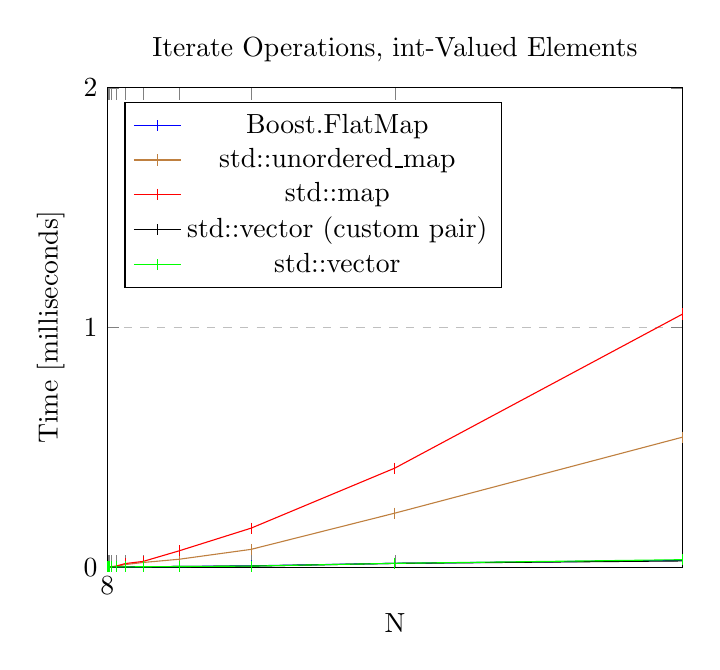
\begin{tikzpicture}
    \begin{axis}[
        width=3.5in,
        title={Iterate Operations, int-Valued Elements},
        xlabel={N},
        ylabel={Time [milliseconds]},
        xmin=0, xmax=32768,
        ymin=0, ymax=2.0,
        xtick={8,16,32,64,128,256,512,1024,2048,4096,8192,16384,32768,65536},
        xticklabels={8,,,,,,,,,,,,,},
        ytick={0.0,1.0,2.0,3.0},
        legend pos=north west,
        ymajorgrids=true,
        grid style=dashed,
        scaled x ticks=false,
        scaled y ticks=true,
        legend entries={Boost.FlatMap,std::unordered\_map,std::map,std::vector (custom pair),std::vector},
        ]

    \addplot[color=blue,mark=|,]
        coordinates {(8,0.0005726)(16,0.0006978)(32,0.0007122)(64,0.0008242)(128,0.0006284)(256,0.0006424)(512,0.0007404)(1024,0.0010898)(2048,0.0015508)(4096,0.0024444)(8192,0.0051822)(16384,0.0157284)(32768,0.0281318)};

    \addplot[color=brown,mark=|,]
        coordinates {(8,0.0006984)(16,0.0006984)(32,0.0007966)(64,0.0008804)(128,0.0008938)(256,0.001369)(512,0.0025422)(1024,0.0105462)(2048,0.0192482)(4096,0.0327554)(8192,0.074004)(16384,0.22528)(32768,0.542443)};

    \addplot[color=red,mark=|,]
        coordinates {(8,0.0006986)(16,0.0007266)(32,0.0008384)(64,0.0011732)(128,0.001215)(256,0.0020678)(512,0.0041346)(1024,0.0147088)(2048,0.02376)(4096,0.0678718)(8192,0.162493)(16384,0.413348)(32768,1.05622)};

    \addplot[color=black,mark=|,]
        coordinates {(8,0.0006986)(16,0.0006704)(32,0.0006288)(64,0.0005866)(128,0.0006004)(256,0.0006564)(512,0.0007542)(1024,0.0009636)(2048,0.0013968)(4096,0.0025278)(8192,0.0042044)(16384,0.0155748)(32768,0.0258552)};

    \addplot[color=green,mark=|,]
        coordinates {(8,0.0006982)(16,0.0006708)(32,0.0006146)(64,0.0008242)(128,0.0006142)(256,0.0006566)(512,0.0008938)(1024,0.0009638)(2048,0.0014526)(4096,0.0024444)(8192,0.0041488)(16384,0.0157142)(32768,0.030912)};

    \end{axis}
\end{tikzpicture}
\end{center}


For all variants but \code{map}, iteration is relatively similar, and much
faster that \code{map}'s.

\begin{center}
    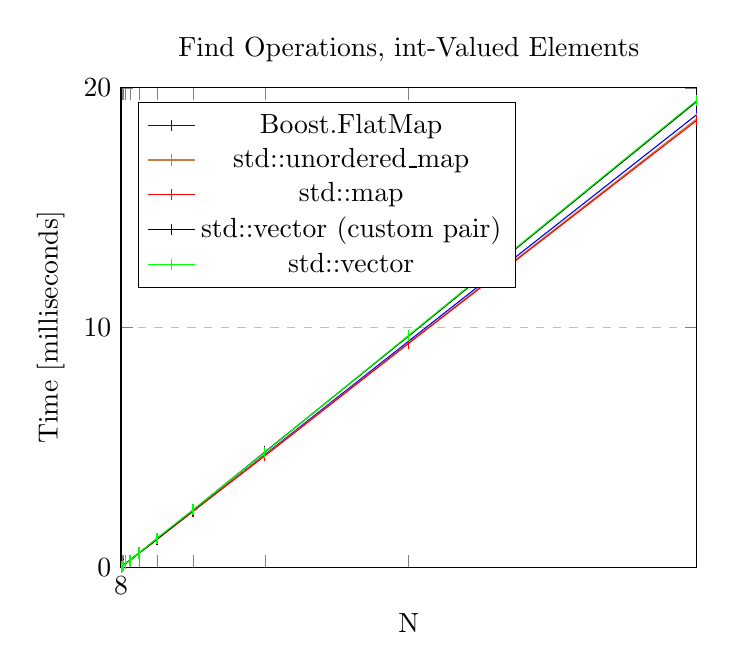
\begin{tikzpicture}
    \begin{axis}[
        width=3.5in,
        title={Find Operations, int-Valued Elements},
        xlabel={N},
        ylabel={Time [milliseconds]},
        xmin=0, xmax=32768,
        ymin=0, ymax=20.0,
        xtick={8,16,32,64,128,256,512,1024,2048,4096,8192,16384,32768,65536},
        xticklabels={8,,,,,,,,,,,,,},
        ytick={0.0,10.0,20.0,30.0},
        legend pos=north west,
        ymajorgrids=true,
        grid style=dashed,
        scaled x ticks=false,
        scaled y ticks=true,
        legend entries={Boost.FlatMap,std::unordered\_map,std::map,std::vector (custom pair),std::vector},
        ]

    \addplot[color=blue,mark=|,]
        coordinates {(8,0.0051258)(16,0.009932)(32,0.0192062)(64,0.038221)(128,0.0743394)(256,0.150843)(512,0.28994)(1024,0.586391)(2048,1.17648)(4096,2.32164)(8192,4.69452)(16384,9.43365)(32768,18.8765)};

    \addplot[color=brown,mark=|,]
        coordinates {(8,0.0051824)(16,0.009819)(32,0.0195278)(64,0.0364302)(128,0.0725802)(256,0.144877)(512,0.291712)(1024,0.587129)(2048,1.17517)(4096,2.33754)(8192,4.66846)(16384,9.36018)(32768,18.705)};

    \addplot[color=red,mark=|,]
        coordinates {(8,0.0050006)(16,0.0099736)(32,0.0189266)(64,0.0381332)(128,0.0721886)(256,0.146389)(512,0.287871)(1024,0.578356)(2048,1.15164)(4096,2.33619)(8192,4.64242)(16384,9.34145)(32768,18.6374)};

    \addplot[color=black,mark=|,]
        coordinates {(8,0.0049584)(16,0.0097354)(32,0.0191222)(64,0.036499)(128,0.107572)(256,0.147548)(512,0.2904)(1024,0.585499)(2048,1.1704)(4096,2.37682)(8192,4.8034)(16384,9.64918)(32768,19.4283)};

    \addplot[color=green,mark=|,]
        coordinates {(8,0.005084)(16,0.0100706)(32,0.0196674)(64,0.0361632)(128,0.0723416)(256,0.144362)(512,0.294509)(1024,0.586093)(2048,1.20946)(4096,2.38596)(8192,4.78721)(16384,9.67802)(32768,19.4717)};

    \end{axis}
\end{tikzpicture}
\end{center}


\code{find()} performance is roughly similar across all the
implementations, and they all show superlinear growth.  Note that
Boost.FlatMap performs the best here.

\begin{center}
    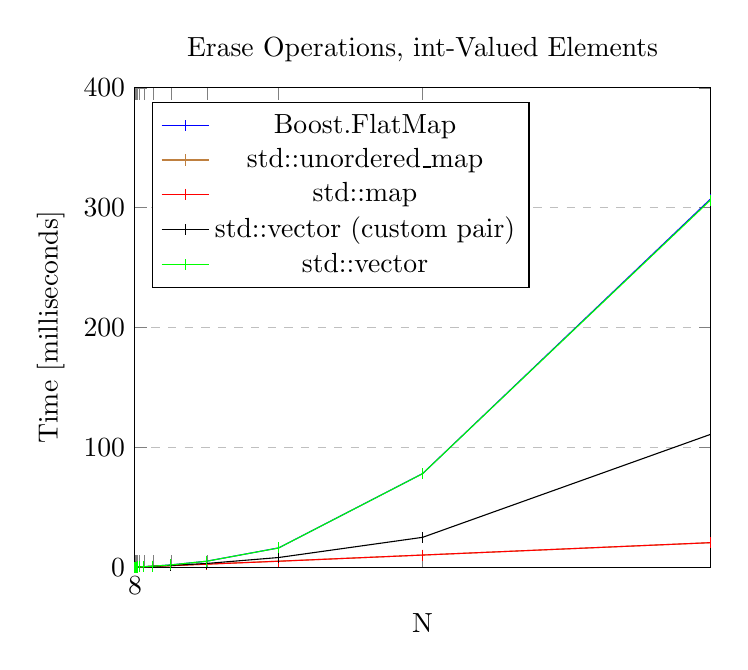
\begin{tikzpicture}
    \begin{axis}[
        width=3.5in,
        title={Erase Operations, int-Valued Elements},
        xlabel={N},
        ylabel={Time [milliseconds]},
        xmin=0, xmax=32768,
        ymin=0, ymax=400.0,
        xtick={8,16,32,64,128,256,512,1024,2048,4096,8192,16384,32768,65536},
        xticklabels={8,,,,,,,,,,,,,},
        ytick={0.0,100.0,200.0,300.0,400.0,500.0},
        legend pos=north west,
        ymajorgrids=true,
        grid style=dashed,
        scaled x ticks=false,
        scaled y ticks=true,
        legend entries={Boost.FlatMap,std::unordered\_map,std::map,std::vector (custom pair),std::vector},
        ]

    \addplot[color=blue,mark=|,]
        coordinates {(8,0.0052938)(16,0.009875)(32,0.0197792)(64,0.040256)(128,0.0749262)(256,0.160385)(512,0.332148)(1024,0.749541)(2048,1.82341)(4096,4.91378)(8192,16.0423)(16384,78.0353)(32768,307.115)};

    \addplot[color=brown,mark=|,]
        coordinates {(8,0.005518)(16,0.0106024)(32,0.0215244)(64,0.038468)(128,0.076643)(256,0.152434)(512,0.305643)(1024,0.61665)(2048,1.22388)(4096,2.47594)(8192,4.95881)(16384,10.035)(32768,20.344)};

    \addplot[color=red,mark=|,]
        coordinates {(8,0.005224)(16,0.0104906)(32,0.0200156)(64,0.036961)(128,0.0749108)(256,0.147936)(512,0.300013)(1024,0.603191)(2048,1.20882)(4096,2.43684)(8192,4.87379)(16384,10.0562)(32768,20.3917)};

    \addplot[color=black,mark=|,]
        coordinates {(8,0.0049448)(16,0.0097916)(32,0.0193604)(64,0.0369046)(128,0.079719)(256,0.146975)(512,0.303422)(1024,0.631629)(2048,1.35059)(4096,3.04038)(8192,7.99865)(16384,24.8397)(32768,110.724)};

    \addplot[color=green,mark=|,]
        coordinates {(8,0.0049728)(16,0.009918)(32,0.0194576)(64,0.0396148)(128,0.0795618)(256,0.159294)(512,0.331455)(1024,0.740411)(2048,1.81269)(4096,4.91325)(8192,15.982)(16384,77.987)(32768,306.231)};

    \end{axis}
\end{tikzpicture}
\end{center}


Erasure has a similar performance profile to insertion, except that the sorted
\code{vector<pair<int, int>>} performs substantially better than
Boost.FlatMap.\\


\subsection{Implications}

TODO Iteration is vastly cheaper for contiguous-storage variants.  It has been
suggested that a \code{map} with a custom allocator can achieve similar
performance to flat data structures, but this would not apply to iteration
performance, unless the values were added to the \code{map} in sorted order.\\

In all the graphs above, the reason the custom-\code{pair} sorted vector
performs so much better than \code{vector<pair<int, int>>} seems to be that
the custom-\code{pair} type has \code{nothrow} special functions.
Implementing all the special functions and adding \code{nothrow(false)} to
each makes the custom-\code{pair} version perform identically to the
\code{pair<int, int>} version.

Boost.FlatMap differs quite a bit from a sorted \code{vector}.  Clearly there
are a lot of QOI choices to make in implementing a standard \code{flat_map}.
